%FROM SANGBAEK
During RG-A data taking, the event was triggered in parallel by three physics trigger systems: (1) the electron trigger, (2) photoproduction trigger and (3) opposite sector trigger. This analysis focuses on the (inclusive) electron trigger that is designed to record events with FD electron candidates with minimum $n_{phe}$, $E_{dep.}$, $E_{dep.} PCAL$ conditions and the geometrical matching between detector subsystems. The electron trigger search was adjusted and performed in parallel for each sector. The electron trigger system is highly efficient with 99.5\% trigger efficiency and 95\% DAQ livetime for trigger electrons of momentum above 2 GeV/c. The desired event rate for the RG-A experiment is about 20 kHz, which was estimated using the simulation. This can be easily achieved by the CLAS12 trigger logic with the effective performance level up to 200 kHz \parencite{Raydo2020TheSystem}. The events triggered by the electron trigger has trigger bits ``1'' (True) in any of bits 0 to 6, where the bits 1–6 stan for each sector and 0 is their OR. The trigger bits can be accessed offline. Processing all saved inclusive events is not efficient in many aspects. There are a lot more inclusive events than the exclusive channels of interest, namely DVCS and DV$\pi^0$P. The RG-A has a few skimming modes, trains and wagons, to be commonly used for some specific channels. A train is a coarse skimming, such as the inclusive skim, which requires an electron-proton pair in one event. A wagon is a relatively finer skimming, such as the DVCS wagon, which requires one electron-proton-photon set with some level of DVCS exclusivity. The series of skimming processes is called data cooking. In this analysis, for the base data set we take the DVCS wagon that selects the DVCS candidates with loose exclusivity cuts, and require at least one $e'p'\gamma$ set in the event \sangsite{158} (see Section 3.3 for the cut conditions). The raw data is stored in the HIPO format \sangsite{151} for the entire CLAS collaboration. The HIPO format has the advantages of fast Input/Output (I/O) speed, and compatibility with the Event I/O (EVIO) format that is commonly used for the Jefferson Lab event storage  \parencite{Wolin2007EVIOPackage}. For this analysis, the python program with pandas library was taken as the main analysis tool in that python is supported by modern statistical packages \sangsite{160,161} that are well maintained. This motivates operation of a custom pipeline to convert the data format to pickle, which is the python standard data format \sangsite{162}. We use the CLAS12ROOT \sangsite{163}, a software package to read the HIPO format in C++ and store the related information in ROOT format \sangsite{164}. The ROOT formatted data is once again converted to pickle format, using the uproot library \sangsite{165}. By doing so, the data are reduced into $M \times N$ dimensionality, where $M$ is the number of events, and $N$ is the number of physical quantities and other information that are related (Fig. 2-16). Different data formats have advantages in different stages of data processing. We filter the base data with the PID cuts introduced at Section 2.4 and save in another HIPO format, because the base data contains all detector responses. The filtered HIPO files are converted into ROOT format. Finally, we execute the python script to select DVCS and DV$\pi^0$P events with tighter Event Selection criteria that will be described at 3.3 and save them in the pickle format.



Cooked hipo - PID cuts - filtered hipo - converting - converted root - dvep cuts - exclusive pickle





here we talk about CLAS PID




cross section that requires the coincidence detection of electron, proton,
and photon.

\subsection{Decoding and Track Reconstruction}\label{sec:decrec}

\subsection{Particle Identification}
**photon cuts:
pid 22, status > 2000 (in FD or CD, not ftagger)
momentum greater than 400 MeV each

**proton cuts: pid 2212

**electron cuts: pid==1 and status < 0(negative particle

sangbaek lee thesis \parencite{Lee2022MeasurementDetector}

For this analysis all final state particles should be detected.
After $\pi^0$ decay we are going to have 4 particles: electron, proton and two photons.
The particle identification methods are applied to select the exclusive event with at least one electron, proton and two photons. 


    \subsubsection{Electron}
    \subsubsection{Proton}
    \subsubsection{Photon}
    \subsubsection{Pion}
    
    Basic event builder cuts are utilized, then additional cuts are made that are common with the RGA Analysis note (\href{https://www.overleaf.com/project/5ea737720942930001ff5e9c}{overleaf link} and developed by Sangbaek Lee (sangbaek@mit.edu - \href{https://github.com/Sangbaek/analysis_code/tree/analysis/pid}{github code here}. For this analysis, both the central detector and forward detector are utilized for proton tracking. The forward tagger is also utilized for photon identification. 
    


\subsubsection{Neutral pion}
    In addition to individual particle PID procedures the cut on the mass of two photons is applied:
    \begin{itemize}
    	\item $0.07<M_{\gamma\gamma}<0.2$ GeV
    \end{itemize}
    The pion is more thoroughly constrained by the exclusivity cuts, described in the next section.
    

\begin{figure}[hbt]
	\centering
	\includegraphics[page=6,width=0.6\textwidth]{Chapters/Ch2-Experiment/recon_pid/pid_figs/eppi0.exclusive.pdf}
	
	\caption{The distribution for mass of two photons $M_{\gamma\gamma}$}.
	\label{fig:ggmass}
	
	\centering
	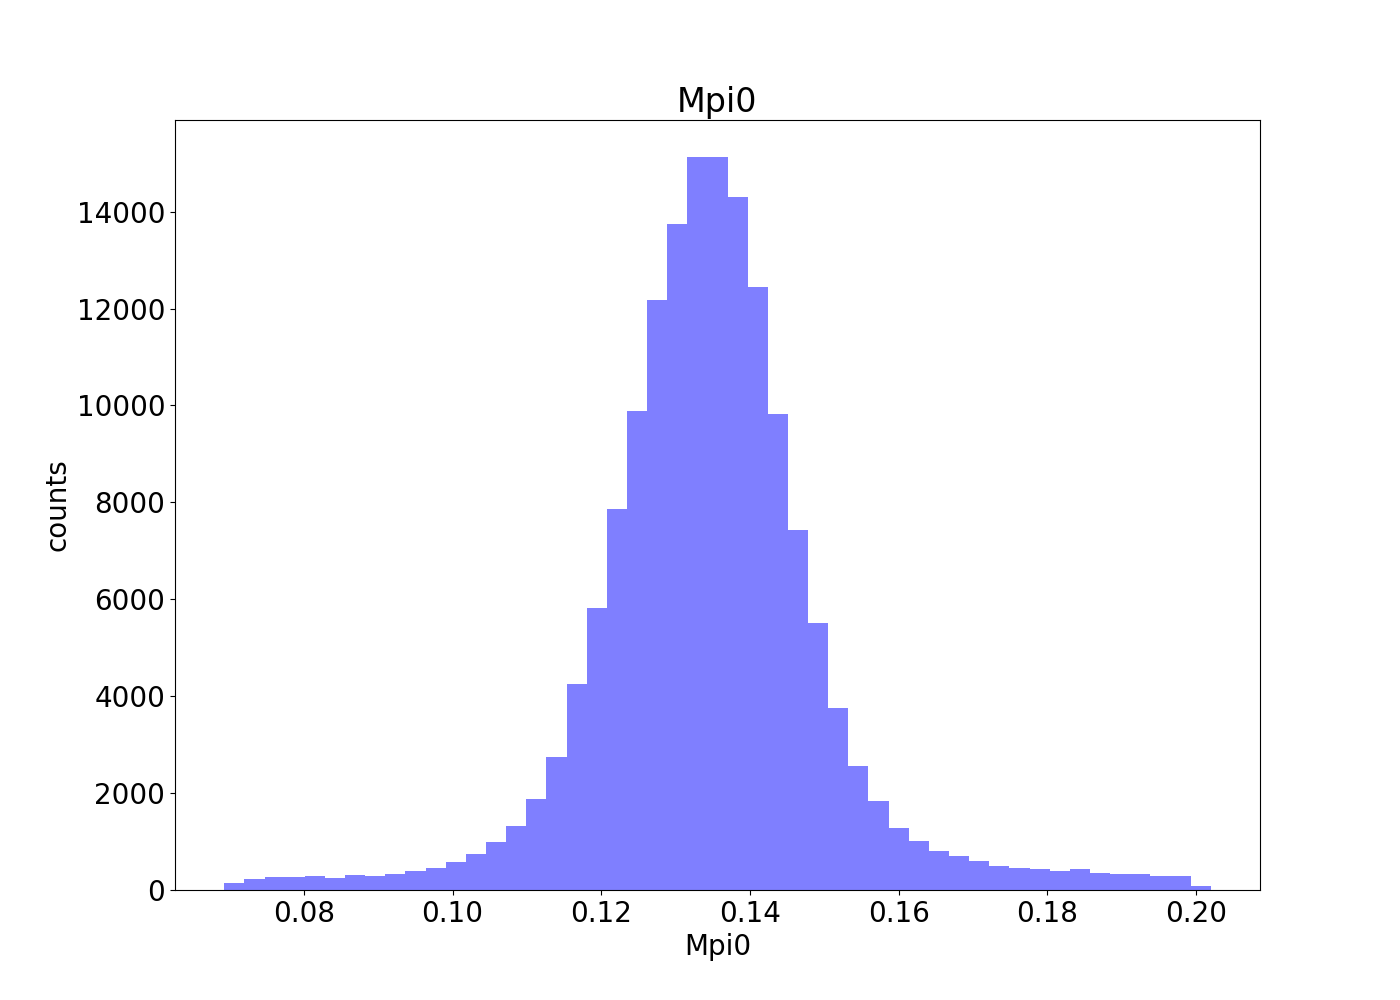
\includegraphics[width=0.6\textwidth]{Chapters/Ch2-Experiment/recon_pid/pid_figs/Mpi0.png}
	
	\caption{The distribution for mass of two photons after exclusivity cuts}.
	\label{fig:ggmass_after}
	
\end{figure}




\subsection{Data Storage and Formatting}
    \subsubsection{Data Location and Availability}
    \subsubsection{File Formatting and Conversion}\label{sec:filtering}
        Mention that same transformations are used for rec events and filtering
    
